\documentclass[nonCC,biblatex=numeric]{GeM-UPM}

%%%%%%%%%%%%%%%%%%%%%%%%%%%%%%%%%%%%%%%%%%%%%%%%%%%%%%%%%%%%%%%%%%%%%%%%
% DATOS DEL PROYECTO
%%%%%%%%%%%%%%%%%%%%%%%%%%%%%%%%%%%%%%%%%%%%%%%%%%%%%%%%%%%%%%%%%%%%%%%%

\title{Evolución de un campo escalar masivo alrededor de un agujero negro de Schwarzschild}

\author{
Alejandro Gragera Serradilla\\
Rocío María Muñoz Guitart\\
Yang Liu\\
Wenyan Xu Ji
}

% Información bibliográfica de los autores
\bibauthor{
Gragera Serradilla, Alejandro \and
Muñoz Guitart, Rocío María \and
Liu, Yang \and
Xu Ji, Wenyan
}

\tutor{Paulo Nicanor Seminario Huertas}

% No se incluye fecha.


%%%%%%%%%%%%%%%%%%%%%%%%%%%%%%%%%%%%%%%%%%%%%%%%%%%%%%%%%%%%%%%%%%%%%%%%
% ENTORNOS MATEMÁTICOS
%%%%%%%%%%%%%%%%%%%%%%%%%%%%%%%%%%%%%%%%%%%%%%%%%%%%%%%%%%%%%%%%%%%%%%%%

\newtheoremstyle{theoremGeM}
  {\topsep}
  {\topsep}
  {\itshape}
  {0pt}
  {\bfseries\color{schoolcolor}}
  {.}
  { }
  {\thmname{#1}\thmnumber{ #2}\textnormal{\thmnote{ (#3)}}}

\theoremstyle{theoremGeM}
\newtheorem{thm}{Teorema}[chapter]
\newtheorem{prop}[thm]{Proposición}
\newtheorem{lem}[thm]{Lema}

\AtBeginDocument{
    \renewcommand*{\proofname}{\color{schoolcolor}Demostración}
}

\newtheoremstyle{remarkGeM}
  {\topsep}
  {\topsep}
  {}
  {0pt}
  {\itshape\color{schoolcolor}}
  {.}
  { }
  {\thmname{#1}\thmnumber{ #2}\textnormal{\thmnote{ (#3)}}}

\theoremstyle{remarkGeM}
\newtheorem*{rmk}{Observación}
\newtheorem{exm}[thm]{Ejemplo}

\newtheoremstyle{definitionGeM}
  {\topsep}
  {\topsep}
  {}
  {0pt}
  {\bfseries\color{schoolcolor}}
  {.}
  { }
  {\thmname{#1}\thmnumber{ #2}\textnormal{\thmnote{ (#3)}}}

\theoremstyle{definitionGeM}
\newtheorem{defn}[thm]{Definición}


%%%%%%%%%%%%%%%%%%%%%%%%%%%%%%%%%%%%%%%%%%%%%%%%%%%%%%%%%%%%%%%%%%%%%%%%
% RESUMEN
%%%%%%%%%%%%%%%%%%%%%%%%%%%%%%%%%%%%%%%%%%%%%%%%%%%%%%%%%%%%%%%%%%%%%%%%

\abstract{spanish}{
Este proyecto estudia la dinámica de un campo escalar masivo en espacio-tiempo
plano y en la geometría de un agujero negro de Schwarzschild. En una primera
etapa se analiza numéricamente la ecuación de Klein--Gordon en espacio plano
y se comprueba su relación de dispersión. Posteriormente, se introduce la
geometría de Schwarzschild y se reduce el problema mediante la simetría
esférica y el uso de la coordenada tortuga.

El objetivo principal es estudiar la aparición de estados cuasi-ligados del
campo escalar alrededor del agujero negro. Estos estados satisfacen condiciones
de contorno físicamente determinadas: comportamiento puramente entrante en el
horizonte de sucesos y decaimiento espacial en el infinito. Como consecuencia,
sus frecuencias son en general complejas y, en el caso de Schwarzschild, su
parte imaginaria es negativa, lo que corresponde a modos que decaen con el
tiempo.

El problema se abordará tanto mediante la evolución temporal de la ecuación
de Klein--Gordon como mediante la formulación de un problema de autovalores
para la ecuación radial. La comparación entre ambos enfoques permitirá
relacionar directamente la dinámica observada en las simulaciones con las
autofrecuencias de los estados cuasi-ligados.
}

\keywords{spanish}{
    Ecuación de Klein--Gordon;
    Agujero negro de Schwarzschild;
    Estados cuasi-ligados;
    Ecuaciones en derivadas parciales;
    Métodos numéricos
}


%%%%%%%%%%%%%%%%%%%%%%%%%%%%%%%%%%%%%%%%%%%%%%%%%%%%%%%%%%%%%%%%%%%%%%%%
% ABSTRACT
%%%%%%%%%%%%%%%%%%%%%%%%%%%%%%%%%%%%%%%%%%%%%%%%%%%%%%%%%%%%%%%%%%%%%%%%

\abstract{english}{
This project studies the dynamics of a massive scalar field in flat spacetime
and in the geometry of a Schwarzschild black hole. First, the Klein--Gordon
equation is analysed numerically in flat spacetime and its dispersion relation
is verified. The Schwarzschild geometry is then introduced, and the problem
is reduced by exploiting spherical symmetry and using the tortoise coordinate.

The main objective is to study the appearance of quasi-bound states of the
scalar field around the black hole. These states satisfy physically motivated
boundary conditions: purely ingoing behaviour at the event horizon and
spatial decay at infinity. As a consequence, their frequencies are generally
complex and, in the Schwarzschild case, their imaginary part is negative,
corresponding to modes that decay with time.

The problem will be approached both through the time evolution of the
Klein--Gordon equation and through an eigenvalue formulation of the radial
equation. Comparing both approaches will make it possible to directly relate
the dynamics observed in the simulations to the eigenfrequencies of the
quasi-bound states.
}

\keywords{english}{
    Klein--Gordon equation;
    Schwarzschild black hole;
    Quasi-bound states;
    Partial differential equations;
    Numerical methods
}


%%%%%%%%%%%%%%%%%%%%%%%%%%%%%%%%%%%%%%%%%%%%%%%%%%%%%%%%%%%%%%%%%%%%%%%%
% DOCUMENTO
%%%%%%%%%%%%%%%%%%%%%%%%%%%%%%%%%%%%%%%%%%%%%%%%%%%%%%%%%%%%%%%%%%%%%%%%

\begin{document}

\nocite{*}


% Capítulos principales
% !TEX root = ../main.tex

\chapter{Introducción}
\label{ch:introduccion}
Este documento en formato {\sffamily pdf} acompaña a otras dos carpetas que contienen material \LaTeX: \texttt{Portada TFG-GEM} y \texttt{Plantilla TFG-GEM}. 

La primera carpeta, \texttt{Portada TFG-GEM}, contiene  logotipos de la UPM, la EPES y el GeM, junto con dos ficheros \LaTeX~ que sirven para configurar la portada del trabajo fin de grado (TFG), incluyendo el título, los nombres del autor y de los tutores, además de la fecha. También aparecen configuradas ---para quien desee añadirlas--- una contraportada y una licencia Creative Commons, necesaria para publicar el trabajo en el repositorio de la UPM.

La segunda carpeta, \texttt{Plantilla TFG-GEM}, contiene lo anterior más una plantilla completa para redactar el TFG en formato \LaTeX~, la cual incluye un fichero de estilo propio: \texttt{GEM-UPM.cls}. Como se puede fácilmente suponer de la lectura de las primeras páginas, esta documentación sigue el mismo formato de la plantilla, por lo que sirve para hacerse una idea del resultado final que se puede esperar. La razón para no tomar este documento como la plantilla misma ---aunque tienen muchos elementos en común--- es que utiliza el paquete \texttt{minted}, cuyo propósito es introducir líneas de código dentro del texto. El uso de \texttt{minted} lleva aparejado una serie de procesos bastante elaborados ---como, por ejemplo, una llamada a Python---, lo cual hace aconsejable que no aparezca en la plantilla en una primera instancia. No obstante lo anterior, \texttt{minted} está cargado en el fichero de estilo y en la sección \ref{s:minted} se darán todas las instrucciones necesarias para su uso.

La plantilla puede compilarse en la plataforma Overleaf. Simplemente recuerda que, en ocasiones, para que la compilación no dé errores, es necesario llevarla a cabo desde el fichero principal, que en este caso se llama \texttt{main.tex}. 

Si compilas los ficheros en local fuera de la plataforma Overleaf, ten en cuenta que el fichero de estilo \texttt{GeM-UPM.cls} requiere usar el motor de compilación pdf\LaTeX~ y, posiblemente, compilar varias veces para que se ejecuten los índices y se actualice la bibliografía. Además, comprueba que la codificación de los caracteres en el procesador de texto que utilices es la estándar; es decir, UTF-8,  y no la obsoleta Latin-1. Por último, en el caso de usar el programa TeXShop en un ordenador Mac, es necesario utilizar el motor de compilación pdf\LaTeX mk.



% !TEX root = ../main.tex

\chapter{Fundamentos físicos y matemáticos}

La carpeta \texttt{Plantilla TFG-GEM} consta de varios ficheros y subcarpetas. Aunque su estructura puede parecer compleja a primera vista, facilita mucho la organización de la memoria. El listado de los diferentes elementos es el siguiente.
\begin{itemize}
    \item \texttt{./appendices/}: carpeta donde se incluyen los ficheros \LaTeX~ de los diferentes apéndices o anexos que aparecen al final de la memoria, en caso de que se quieran utilizar.
    \item \texttt{./chapters/}: carpeta donde se incluyen los ficheros \LaTeX~ de los capítulos que forman parte del cuerpo de la memoria.
    \item \texttt{./figures/}: carpeta donde se incluyen las figuras (imágenes, diagramas) que se usarán a lo largo de todo el documento.
    \item \texttt{./logos/}: carpeta que contiene los logotipos de la Universidad Politécnica de Madrid, de la Escuela Politécnica de Enseñanza Superior y del Grado en Matemáticas. Esta carpeta se utiliza en el fichero de estilo \texttt{GeM-UPM.cls}, por lo que es aconsejable no cambiarla de ubicación o nombre.
    \item \texttt{./GeM-UPM.cls}: fichero de estilo de la memoria. 
    \item \texttt{./main.tex}: fichero principal a partir del cual se compila todo el trabajo. No conviene cambiarle de nombre porque se utiliza en el fichero de estilo \texttt{GeM-UPM.cls}.
    \item \texttt{./referencias.bib}: fichero que contiene las entradas de la bibliografía a las que se hace referencia en la memoria en formato \hologo{BibTeX}.
    \item \texttt{./referencias.tex}: fichero que contiene las entradas de la bibliografía en formato \LaTeX. Solo es necesario utilizar uno de los dos ficheros que contienen la bibliografía: cuál se use depende del formato elegido; véase la sección~\ref{s:referencias-bibliograficas}
\end{itemize}    

En el caso de que únicamente se quiera utilizar la portada de la plantilla ---y, quizás, añadir la licencia Creative Commons y la contraportada---, hay que utilizar la carpeta \texttt{Portada TFG-GEM}, cuya estructura es mucho más simple que la de la plantilla: contiene la subcarpeta \texttt{logos}, el fichero principal \texttt{main.tex} ---en una versión mucho más reducida que el homónimo fichero de la plantilla--- y otro fichero \LaTeX~ llamado \texttt{portada.tex}, en el que se recopilan los comandos esenciales del fichero de estilo que bastan para configurar la portada. 

%%%%%%%%%%%%%%%%%%%%%%%%%%%%%%%%%%%%
\section{El fichero principal \texttt{main.tex}}

A partir de ahora nos referiremos únicamente a los elementos que aparecen  en la carpeta \texttt{Plantilla TFG-GEM}. 

Nótese que el fichero de estilo carga por defecto la opción \texttt{index}, que crea un índice alfabético, cuestión que se explica en la sección~\ref{s:indice}. Las otras opciones disponibles ---que si se utilizan han de escribirse junto a \texttt{index} separadas por comas--- son
\begin{itemize}
    \item \texttt{nonCC}, que debe ser seleccionada por el autor que no desee que su trabajo tenga licencia Creative Commons, necesaria para publicarlo en el repositorio de la UPM;
    \item \texttt{biblatex}, para escribir la bibliografía en formato \hologo{BibTeX}. Véase la sección~\ref{s:referencias-bibliograficas};
    \item \texttt{minted}, que se usa para insertar código fuente de un lenguaje de programación en el texto; véase la sección~\ref{s:minted}.
\end{itemize} 

%%%%%%%%%%%%%%%%%%%%%%%%%%%%%%%%%%%%%%%%%%%%%%%%%%%%%%%%%%%%%
\section{Bibliografía}
\label{s:referencias-bibliograficas}

Hay muchas formas diferentes de gestionar las referencias bibliográficas. Aquí se ofrecen dos posibilidades.

\subsection{Bibliografía con {\ttfamily biblatex}}
La primera consiste en utilizar el paquete \texttt{biblatex}, que constituye una forma cómoda y simple de manejar la bibliografía. Por defecto, el estilo de las citas es alfabético; véanse \cite{wiles95} y \cite{berger88}.

\subsection{Bibliografía sin {\ttfamily biblatex}}
La otra posibilidad es escribir la bibliografía en el fichero \texttt{referencias.tex} en formato \LaTeX~  y es la que viene cargada por defecto en el fichero de estilo, por lo que, para emplearla, no hay que hacer nada, salvo asegurarse de que no se ha seleccionado la opción \texttt{biblatex} en la primera línea del fichero \texttt{main.tex}. 

%%%%%%%%%%%%%%%%%%%%%%%%%%%%%%%%%%%%%
\section{Índice alfabético}
\label{s:indice}

El índice alfabético es un listado ordenado lexicográficamente que aparece al final de la memoria, formado por aquellas palabras que deseamos destacar o que se encuentren rápidamente.

La inclusión del índice alfabético es opcional; si no se crea ningún término de este tipo, entonces el índice alfabético no se mostrará.


%%%%%%%%%%%%%%%%%%%%%%%%%%%%%%%%%%%%%%%%%%%%%%%%%%%%%%%%%%%%%%%%%%%%%%%%%%%%%%
\section{El fichero de estilo \texttt{GeM-UPM.cls}}\label{s:estilo}
El fichero de estilo \texttt{GeM-UPM.cls} contiene todos los códigos e instrucciones que hacen que el documento, al compilar el fichero \texttt{main.tex}, se vea como es. En general, su manipulación requiere un conocimiento avanzado del lenguaje \LaTeX~  y no se recomienda modificarlo. 



%%%%%%%%%%%%%%%%%%%%%%%%%%%%%%%%%%%%
\section{El paquete \texttt{minted}}\label{s:minted}

A lo largo de este documento se ha hecho un uso frecuente del paquete \texttt{minted} para mencionar diversos comandos de \LaTeX, por lo que parece conveniente dedicar unos comentarios que expliquen brevemente su propósito y funcionamiento. El paquete  \texttt{minted} se usa para añadir el código fuente de múltiples lenguajes de programación a un texto. Este paquete no se carga de manera automática, sino que hay que indicarlo en el preámbulo del fichero como una opción de la plantilla. 

% !TEX root = ../main.tex

\chapter{Otros elementos}
\label{ch:otro}


\section{Figuras y ecuaciones}

Ejemplo de dibujo, véase la figura~\ref{fg:figura}.
\begin{figure}[htb]
\centering	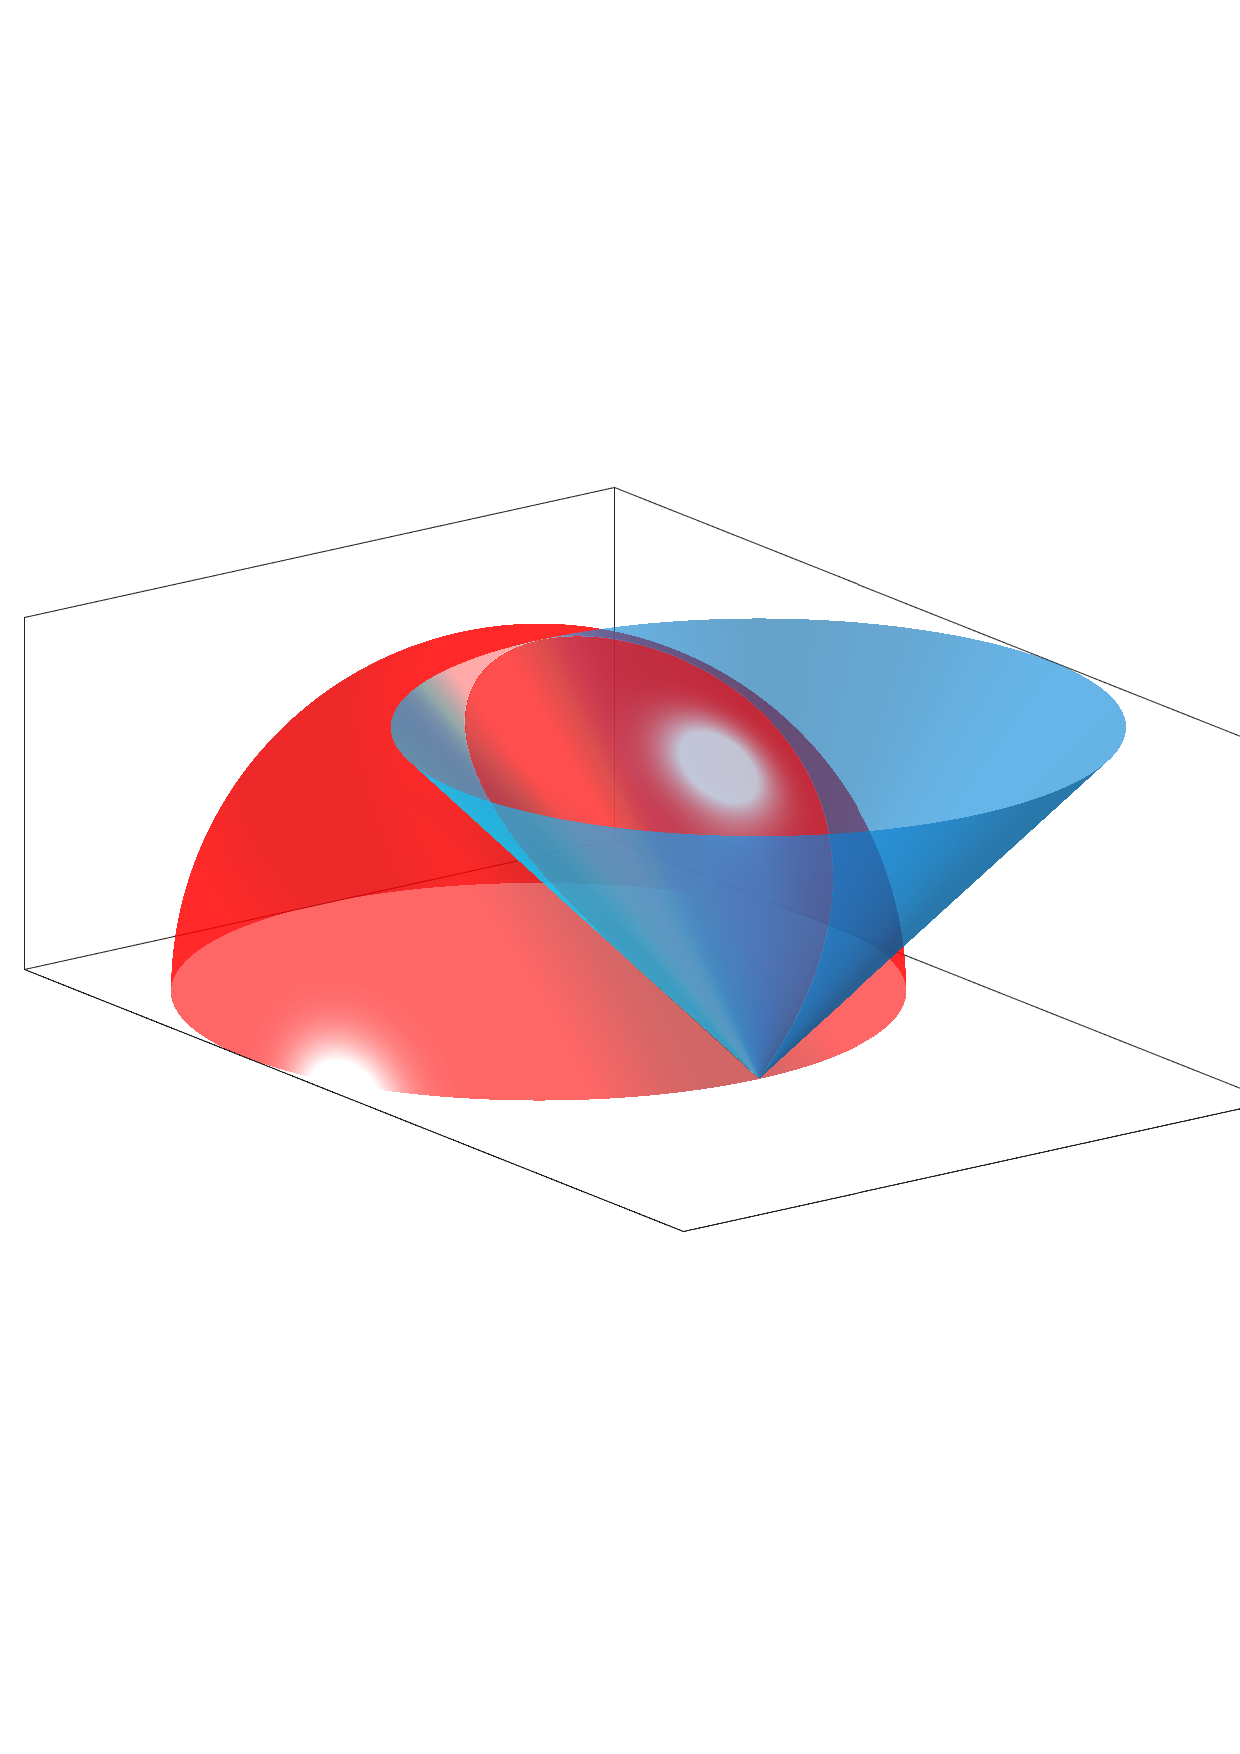
\includegraphics[width=0.5\textwidth]{figures/viviani.pdf}
\caption{Ejemplo de figura.}\label{fg:figura}
\end{figure}

Ejemplo de ecuación. Véase la definición de la función $f$ en~\eqref{fm:formula}.

\begin{equation}\label{fm:formula}
f(x) = \left\{ \begin{array}{ll}
\displaystyle\frac{3}{2}x^2, &  \mbox{si}\; -b \leq x < b; \\[5mm]
\displaystyle\int_{0}^{x} g(t)\, dt,  &  \mbox{resto.}
\end{array}\right.
\end{equation}

\section{Tablas}
Cómo introducir una tabla. Véase la tabla~\ref{tab:mi_etiqueta}.
\begin{table}[ht]
\centering
\begin{tabular}{ccc}
\hline\noalign{\smallskip}
$n$ &$B$ & $S$  \\[1mm]
\hline \noalign{\smallskip}         
 2& $\pi R^2$& $2\pi R$  \\[3mm]
 3& $\displaystyle \frac{4\pi}{3}R^3 $& $4\pi R^2$ \\[3mm]
 \hline \noalign{\smallskip}
\end{tabular}
\caption{Ejemplo de tabla.}
\label{tab:mi_etiqueta}
\end{table}

\section{Definiciones y teoremas}

En la plantilla se han definido entornos para organizar las definiciones y los resultados matemáticos dentro del texto. Estos entornos se hallan en el preámbulo del fichero \verb+main.tex+, para que se puedan modificar si el autor del trabajo prefiere configurarlos de otro modo. A continuación, aparecen algunos ejemplos.
\begin{defn}
    Diremos que un triángulo es \emph{rectángulo}\index{triángulo!rectángulo} si uno de los ángulos es un ángulo recto, esto es, $\tfrac\pi2$. En este triángulo, el lado opuesto al ángulo recto es la \emph{hipotenusa}\index{hipotenusa}, y los otros dos lados se les denomina \emph{catetos}\index{cateto}.

    Cuando en un triángulo, el ángulo de mayor amplitud es mayor que un ángulo recto, diremos que el triángulo es \emph{obtusángulo}\index{triángulo!obtusángulo}; de lo contrario diremos que es \emph{acutángulo}\index{triángulo!acutángulo}.
\end{defn}

\begin{thm}
    En un triángulo rectángulo se cumple la igualdad $a^2=b^2+c^2$, donde $a$ es la longitud de la hipotenusa, y $b$ y $c$ son las longitudes de los catetos.
\end{thm}
\begin{proof}
    Sea $T$ un triángulo rectángulo.
\end{proof}

\begin{rmk}
    La hipotenusa, por definición, es el lado contrario al ángulo recto, pero también coincide con el lado del triángulo de mayor longitud.
\end{rmk}

\begin{exm}
    Las ternas pitagóricas como $(3,4,5)$ son ejemplos de longitudes de los lados de un triángulo rectángulo. En este caso, la longitud de la hipotenusa es~$5$.
\end{exm}

Algunas sugerencias adicionales:
\begin{itemize}
    \item Todas las variables matemáticas deben ir en modo matemático y aparecer en itálicas: ``Sea $X$ el conjunto...''.
    \item En cambio, las funciones comunes como seno, coseno, etc. no deben estar en itálicas: ``Considera la función $f(x)=\sin x$...''.
    \item Evita en lo posible que una ecuación rompa entre dos líneas.
    \item No comiences tus frases con un símbolo (o un número). También eso es deseable para el comienzo de línea.
    \item Destaca una fórmula situándola fuera del texto si al incluirla dentro de la línea de texto normal provoca una separación entre líneas mayor de la diseñada, o cuando se haga referencia a ella en otra parte del texto.
\end{itemize}

Finalmente, se puede usar la letra {\sffamily sin serifa} en el documento para destacar términos.

Las letras griegas más utilizadas son las siguientes:
\[
\alpha,\beta,\gamma,\lambda,\mu
\]
\input{chapters/04_metodologia_numerica}
\input{chapters/05_validacion_espacio_plano}
\input{chapters/06_estados_cuasiligados}
\input{chapters/07_resultados_discusion}
\input{chapters/08_conclusiones}

% Apéndices
\appendix
\input{appendices/A_derivacion_klein_gordon}
\input{appendices/B_reduccion_radial}
\input{appendices/C_detalles_numericos}
\input{appendices/D_unidades}

\end{document}
